\documentclass[border=10pt]{standalone}
\usepackage{tikz}
\usetikzlibrary{shapes.geometric, arrows.meta, positioning, calc, fit, backgrounds, shadows.blur}
\usepackage[T1]{fontenc}
\usepackage{helvet}
\renewcommand{\familydefault}{\sfdefault}

\definecolor{morphorange}{HTML}{FF6B2B}
\definecolor{morphdark}{HTML}{0D0D1A}
\definecolor{morphgray}{HTML}{1A1A2E}
\definecolor{morphblue}{HTML}{4A90D9}
\definecolor{morphpurple}{HTML}{8B5CF6}
\definecolor{morphgreen}{HTML}{10B981}
\definecolor{morphaccent}{HTML}{F59E0B}
\definecolor{textwhite}{HTML}{F0F0F0}
\definecolor{textgray}{HTML}{9CA3AF}

\begin{document}
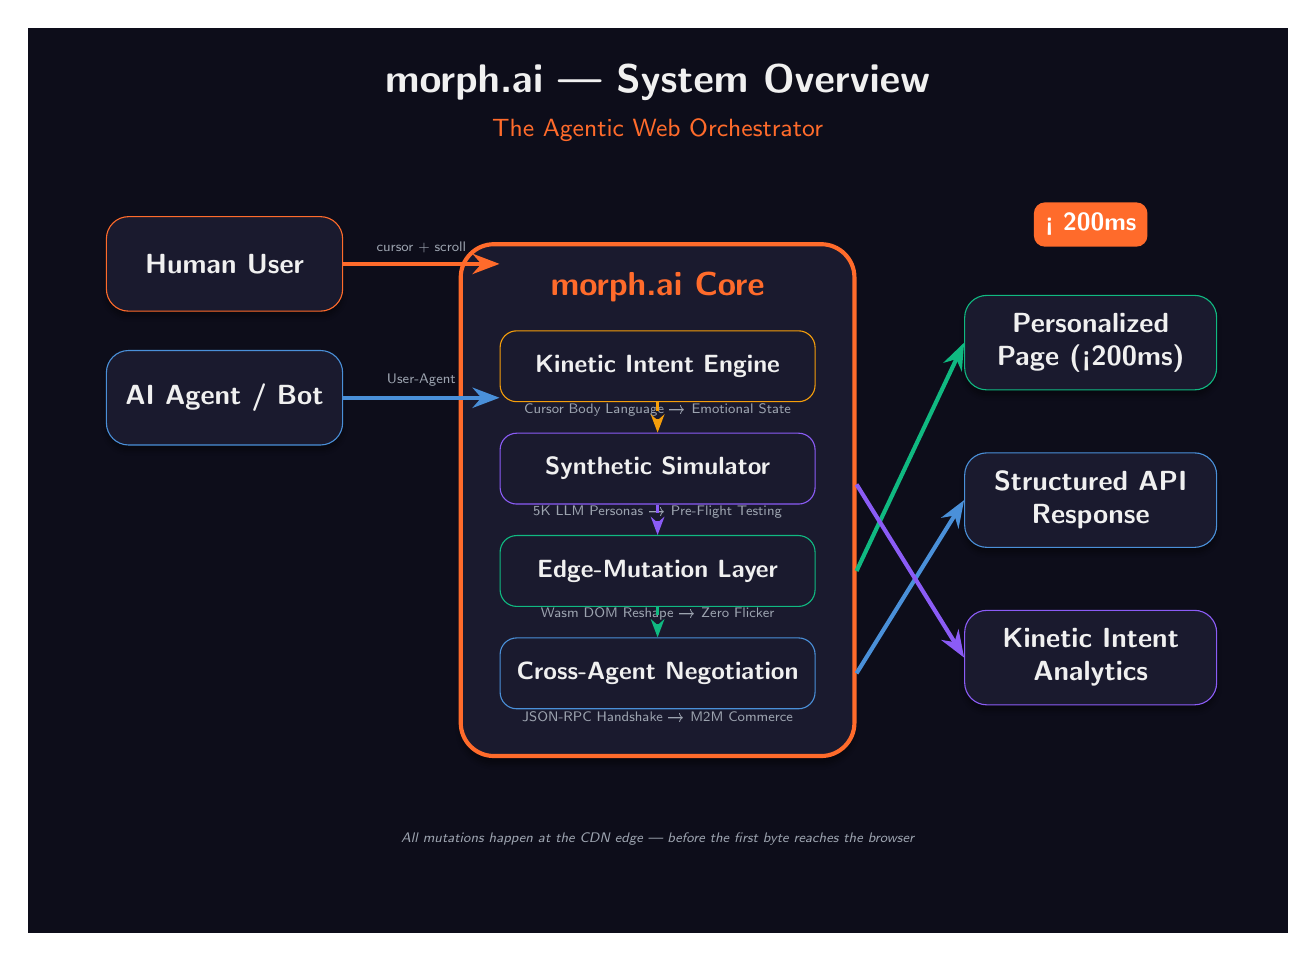
\begin{tikzpicture}[
    every node/.style={font=\sffamily},
    >=Stealth,
]

% Background
\fill[morphdark] (-8,-6) rectangle (8,5.5);

% Title
\node[text=textwhite, font=\sffamily\bfseries\Large] at (0,4.8) {morph.ai — System Overview};
\node[text=morphorange, font=\sffamily\small] at (0,4.2) {The Agentic Web Orchestrator};

% --- Left: User/Agent Input ---
\node[draw=morphorange, fill=morphgray, rounded corners=8pt, minimum width=3cm, minimum height=1.2cm, 
      text=textwhite, font=\sffamily\bfseries, blur shadow={shadow blur steps=5, shadow xshift=0pt, shadow yshift=-2pt}] 
      (user) at (-5.5, 2.5) {Human User};

\node[draw=morphblue, fill=morphgray, rounded corners=8pt, minimum width=3cm, minimum height=1.2cm,
      text=textwhite, font=\sffamily\bfseries, blur shadow={shadow blur steps=5, shadow xshift=0pt, shadow yshift=-2pt}] 
      (agent) at (-5.5, 0.8) {AI Agent / Bot};

% --- Center: morph.ai Core ---
\node[draw=morphorange, fill=morphgray, rounded corners=12pt, minimum width=5cm, minimum height=6.5cm,
      blur shadow={shadow blur steps=8, shadow xshift=0pt, shadow yshift=-3pt}, line width=1.5pt] 
      (core) at (0, -0.5) {};

\node[text=morphorange, font=\sffamily\bfseries\large] at (0, 2.2) {morph.ai Core};

% Core modules
\node[draw=morphaccent, fill=morphgray, rounded corners=6pt, minimum width=4cm, minimum height=0.9cm,
      text=textwhite, font=\sffamily\small\bfseries] 
      (kinetic) at (0, 1.2) {Kinetic Intent Engine};
\node[text=textgray, font=\sffamily\tiny] at (0, 0.65) {Cursor Body Language → Emotional State};

\node[draw=morphpurple, fill=morphgray, rounded corners=6pt, minimum width=4cm, minimum height=0.9cm,
      text=textwhite, font=\sffamily\small\bfseries] 
      (simulator) at (0, -0.1) {Synthetic Simulator};
\node[text=textgray, font=\sffamily\tiny] at (0, -0.65) {5K LLM Personas → Pre-Flight Testing};

\node[draw=morphgreen, fill=morphgray, rounded corners=6pt, minimum width=4cm, minimum height=0.9cm,
      text=textwhite, font=\sffamily\small\bfseries] 
      (edge) at (0, -1.4) {Edge-Mutation Layer};
\node[text=textgray, font=\sffamily\tiny] at (0, -1.95) {Wasm DOM Reshape → Zero Flicker};

\node[draw=morphblue, fill=morphgray, rounded corners=6pt, minimum width=4cm, minimum height=0.9cm,
      text=textwhite, font=\sffamily\small\bfseries] 
      (handshake) at (0, -2.7) {Cross-Agent Negotiation};
\node[text=textgray, font=\sffamily\tiny] at (0, -3.25) {JSON-RPC Handshake → M2M Commerce};

% --- Right: Output ---
\node[draw=morphgreen, fill=morphgray, rounded corners=8pt, minimum width=3.2cm, minimum height=1.2cm,
      text=textwhite, font=\sffamily\bfseries, blur shadow={shadow blur steps=5, shadow xshift=0pt, shadow yshift=-2pt}] 
      (personalized) at (5.5, 1.5) {\begin{tabular}{c}Personalized\\Page (<200ms)\end{tabular}};

\node[draw=morphblue, fill=morphgray, rounded corners=8pt, minimum width=3.2cm, minimum height=1.2cm,
      text=textwhite, font=\sffamily\bfseries, blur shadow={shadow blur steps=5, shadow xshift=0pt, shadow yshift=-2pt}] 
      (apiresponse) at (5.5, -0.5) {\begin{tabular}{c}Structured API\\Response\end{tabular}};

\node[draw=morphpurple, fill=morphgray, rounded corners=8pt, minimum width=3.2cm, minimum height=1.2cm,
      text=textwhite, font=\sffamily\bfseries, blur shadow={shadow blur steps=5, shadow xshift=0pt, shadow yshift=-2pt}] 
      (analytics) at (5.5, -2.5) {\begin{tabular}{c}Kinetic Intent\\Analytics\end{tabular}};

% --- Arrows ---
\draw[->, morphorange, line width=1.5pt] (user.east) -- node[above, text=textgray, font=\tiny] {cursor + scroll} (kinetic.west |- user.east);
\draw[->, morphblue, line width=1.5pt] (agent.east) -- node[above, text=textgray, font=\tiny] {User-Agent} (handshake.west |- agent.east);

\draw[->, morphgreen, line width=1.5pt] (edge.east -| core.east) -- (personalized.west);
\draw[->, morphblue, line width=1.5pt] (handshake.east -| core.east) -- (apiresponse.west);
\draw[->, morphpurple, line width=1.5pt] (kinetic.east -| core.east) ++(0,-1.5) -- (analytics.west);

% Internal arrows
\draw[->, morphaccent, line width=0.8pt, dashed] (kinetic) -- (simulator);
\draw[->, morphpurple, line width=0.8pt, dashed] (simulator) -- (edge);
\draw[->, morphgreen, line width=0.8pt, dashed] (edge) -- (handshake);

% --- Bottom label ---
\node[text=textgray, font=\sffamily\tiny\itshape] at (0, -4.8) {All mutations happen at the CDN edge — before the first byte reaches the browser};

% Latency badge
\node[fill=morphorange, rounded corners=4pt, text=white, font=\sffamily\bfseries\small, inner sep=4pt] 
      at (5.5, 3) {< 200ms};

\end{tikzpicture}
\end{document}
